\documentclass[12pt]{letter}\usepackage[letterpaper,margin=0.65in]{geometry}\usepackage{textcomp}\usepackage{graphicx}\usepackage[rflt]{floatflt}\pagenumbering{gobble}\begin{document}\begin{floatingfigure}{0.15\textwidth}\raisebox{0pt}[0pt][0pt]{\raisebox{-2.5cm}{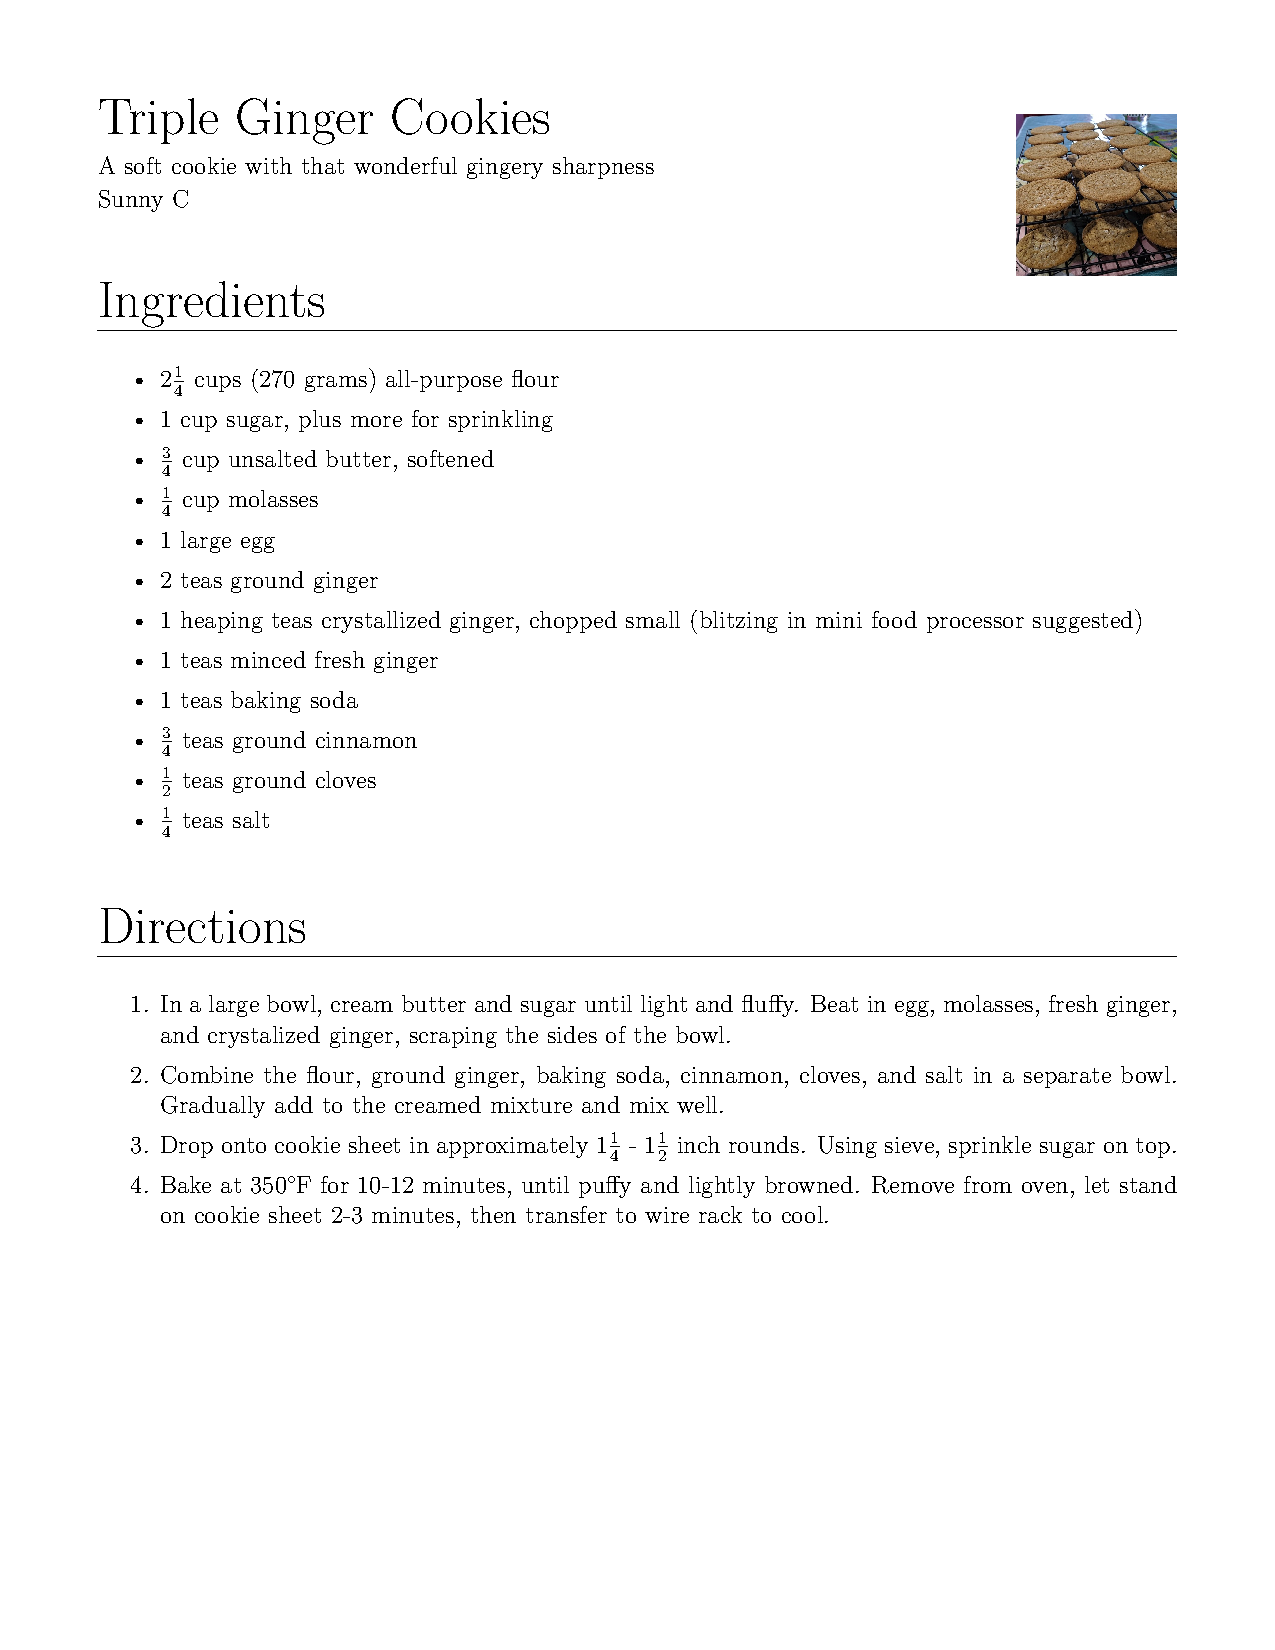
\includegraphics[width=0.15\textwidth]{triple-ginger-cookies}}}\end{floatingfigure}\begin{huge}Triple Ginger Cookies\end{huge}\newline\vspace{-2.5mm}\newline\renewcommand{\arraystretch}{1.1}\begin{tabular*}{\textwidth}{@{\extracolsep{\fill}}lr}A soft cookie with that wonderful gingery sharpness\\Sunny C\end{tabular*}\newline\vspace{10mm}\newline\begin{huge}Ingredients\end{huge}\\\rule[2.8mm]{\textwidth}{.1pt}\vspace{-3mm}\begin{itemize}\item 2$\frac{1}{4}$ cups flour\item 1 cup sugar, plus more for sprinkling\item $\frac{3}{4}$ cup unsalted butter, softened\item $\frac{1}{4}$ cup molasses\item 1 large egg\item 2 teas ground ginger\item 1 heaping teas crystallized ginger, chopped small (blitzing in mini food processor suggested)\item 1 teas minced fresh ginger\item 1 teas baking soda\item $\frac{3}{4}$ teas ground cinnamon\item $\frac{1}{2}$ teas ground cloves\item $\frac{1}{4}$ teas salt\end{itemize}\vspace{7mm}\begin{huge}Directions\end{huge}\\\rule[2.8mm]{\textwidth}{.1pt}\vspace{-3mm}\begin{enumerate}\item In a large bowl, cream butter and sugar until light and fluffy. Beat in egg, molasses, fresh ginger, and crystalized ginger, scraping the sides of the bowl.\item Combine the flour, ground ginger, baking soda, cinnamon, cloves, and salt in a separate bowl. Gradually add to the creamed mixture and mix well.\item Drop onto cookie sheet in approximately 1$\frac{1}{4}$ - 1$\frac{1}{2}$ inch rounds. Using sieve, sprinkle sugar on top.\item Bake at 350\textdegree F for 10-12 minutes, until puffy and lightly browned. Remove from oven, let stand on cookie sheet 2-3 minutes, then transfer to wire rack to cool.\end{enumerate}\end{document}